% This document is part of the EPRVCalibration project
% Copyright 2019 the authors. All rights reserved.

% style notes
% -----------
% - use \acronym and use \eprv, \lfc, and so on.

\documentclass[modern]{aastex63}
\usepackage[ruled,vlined,norelsize]{algorithm2e}

% hogg dealing with his shit
\addtolength{\topmargin}{-0.30in}
\addtolength{\textheight}{0.70in}
\renewcommand{\twocolumngrid}{} % hahaha!
\setlength{\parindent}{1.1\baselineskip}
\sloppy\sloppypar\raggedbottom\frenchspacing
\shorttitle{excalibur: a wavelength-calibration model}
\shortauthors{zhao, hogg, bedell, fischer}

% typesetting words
\newcommand{\project}[1]{\textsl{#1}}
\newcommand{\name}{\project{Excalibur}}
\newcommand{\acronym}[1]{{\small{#1}}}
\newcommand{\expres}{\project{\acronym{EXPRES}}}
\newcommand{\espresso}{\project{\acronym{ESPRESSO}}}
\newcommand{\neid}{\project{\acronym{NEID}}}
\newcommand{\eprv}{\acronym{EPRV}}
\newcommand{\lfc}{\acronym{LFC}}
\newcommand{\code}[1]{\texttt{#1}}
\newcommand{\target}{HD $\bigstar$}

\newcommand{\lz}[1]{\textcolor{orange}{#1}}
\newcommand{\mb}[1]{\textcolor{violet}{#1}}

% math shih
\newcommand{\mps}{\mathrm{m\,s^{-1}}}

\begin{document}
\title{\name:
  A Non-Parametric, Hierarchical \\
  Wavelength-Calibration Method for a Precision Spectrograph}

\correspondingauthor{Lily Zhao}
\email{lily.zhao@yale.edu}

\author[0000-0002-3852-3590]{Lily Zhao}
\affil{Yale University, 52 Hillhouse, New Haven, CT 06511, USA}
\affil{Flatiron Institute, Simons Foundation, 162 Fifth Avenue, New York, NY 10010, USA}

\author[0000-0003-2866-9403]{David W. Hogg}
\affil{Center for Cosmology and Particle Physics, Department of Physics, New York University, 726 Broadway, New York, NY 10003, USA}
\affil{Center for Data Science, New York University, 60 Fifth Avenue, New York, NY 10011, USA}
\affil{Max-Planck-Institut für Astronomie, Königstuhl 17, D-69117 Heidelberg, Germany}
\affil{Flatiron Institute, Simons Foundation, 162 Fifth Avenue, New York, NY 10010, USA}

\author[0000-0001-9907-7742]{Megan Bedell}
\affil{Flatiron Institute, Simons Foundation, 162 Fifth Avenue, New York, NY 10010, USA}

\author[0000-0003-2221-0861]{Debra A. Fischer}
\affil{Yale University, 52 Hillhouse, New Haven, CT 06511, USA}

\begin{abstract}\noindent%
\name\ is a non-parametric, hierarchical framework for precision wavelength-calibration of spectrographs.  This method is designed with the needs of extreme-precision radial velocity (\eprv) in mind, which require that instruments be calibrated or stabilized to better than $10^{-4}$ of a pixel.  Instruments are likely to vary along only a few dominant degrees of freedom, especially \eprv\ instruments with highly stabilized optical systems and detectors.  \name\ takes advantage of this property by using all calibration data to construct a low-dimensional space of all possible calibrations for an instrument.  \name\ also takes advantage of the development of laser-frequency combs or etalons, which generate a dense set of stable calibration points.  This density of calibration lines permits the freedom of a non-parametric wavelength solution that can match or adapt to any instrument or detector oddities, more so than any parametric model.  We demonstrate the success of this method with data from the \textsl{EXtreme PREcision Spectrograph}, \expres, which includes a laser frequency comb.  Using \name\ wavelengths to predict the wavelengths of known calibration lines returns smaller per-line RMS by a factor of 5 when compared to a classic wavelength solution that is constructed using polynomials and treats each exposure individually .  Employing \name\ wavelengths on \expres\ RV measurements of HD 3651 reduced the RMS of a planet fit by \lz{blah}.
\end{abstract}


% Add official keywords
\keywords{instrumentation: spectrographs -- instrumentation: detectors -- techniques: spectroscopic -- techniques: radial velocities -- methods: data analysis -- methods: statistical}

\section{Introduction} 
Precise, radial-velocity (\eprv) programs have been incredibly fruitful in finding and characterizing extra-solar planets \citep[e.g.][]{mayor2011, bonfils2013, plavchan2015, butler2017}.  These programs typically make use of spectrographs with resolutions on the order of $10^5$, which correspond to line widths on the order of $3000\,\mps$.  Exoplanet science happens at the level of $3\,\mps$ precision, which is sensitive enough to discover gas-giant planets around other stars.  The newest generation of instruments aim  to reach $0.1\,\mps$ precision, the required precision to detect terrestrial worlds \citep{fischer2016}.  This requires new spectrographs to be calibrated or stabilized to better than $10^{-4}$ of a pixel (assuming that the spectrographs are well sampled).    Some hardware--software systems, such as \espresso, \expres,  \neid, etc., were designed to deliver precision at this level \citep{pepe2013,  jurgenson2016, neid}.  Early data from \expres\ and \espresso\ suggest that the hardware improvements truly propagate through to sub-$\mps$ uncertainties on final, on-sky RV measurements \citep{blackman2020, petersburg2020, mascareno2020}.

Traditionally, wavelength solutions are constructed by fitting a polynomial to lines from a calibration source to describe the relationship between wavelength and pixel for each echelle order \citep{butler1996, lovis2007, cersullo2019}.  In this framework, each calibration image is treated independently.  The returned wavelength solutions worked well at the level of 1 $\mps$ precision.  The move towards 0.1 $\mps$ RV precision, however, necessitates higher-fidelity calibration data and wavelength models.  These models need to account for high-order spatial variations that can arise from small imperfections in the optics of an instrument and non-uniformity in detector pixel sizes/spacing.  There has been significant effort in using an entire set of calibration images to identify incongruous ThAr lines \citep{coffinet2019} or obtain high-resolution Fourier transform spectra of reference cells \citep{wang2020}.  It has also been found that using a segmented polynomial in the dispersion direction, tuned to capture detector defects, better describes the wavelength solution than a single, continuous polynomial \citep{milakovic2020}.

Here, we propose to simplify and improve calibration programs for \eprv\ hardware systems with two practical yet innovative ideas.  The first flows from the fact that calibration sources---which include arc lamps (in some wavelength ranges), etalons, and laser-frequency combs (\lfc s)---illuminate the spectrograph with very stable, very dense sets of lines; almost every location in the spectrograph image plane is surrounded by nearby, useful calibration lines.

This recommends a calibration methodology that is \emph{non-parametric}, or not defined by a prescribed, analytic function described by a finite number of parameters :  If every point in the spectrograph detector is sufficiently surrounded by nearby calibration lines, the wavelength solution can, for example, be made simply as an interpolation of the calibration data.  The density of lines removes the need to enforce any functional form for the wavelength solution (such as a continuous ninth-order polynomial, for example).  In some ways, this is a generalization of the recent work that demonstrated the efficacy of constructing a wavelength solution as multiple, segmented polynomials \citep{milakovic2020}.  Going non-parametric will improve calibration accuracy by not forcing the choice of a parametric form that may bias the calibration, especially when the chosen function is inappropriate (as, for example, polynomials are at detector edges).

The second simple idea follows from the observation that most physical systems have only a few dominant degrees of freedom, meaning most spectrographs vary along only a small number of axes in ``calibration space'', or the (very high-dimensional) space of all possible wavelength solutions.  This is particularly likely with the latest generation of \eprv\ instruments that are equipped with stringent environmental stabilizing, likely reducing the number and extent of the axes along which the instrument can vary.  That is, spectrographs, especially stabilized ones, should have few environmentally accessible degrees of freedom.  This renders it inadvisable to fit each calibration exposure or calibrate each science exposure independently.  Instead, all the calibration data (or all the data) should be used to determine the calibration space in which the instrument can and does vary.  Subsequent calibration work then need only determine where in the small, accessible part of calibration space the spectrograph was located for each exposure.

In the context of probabilistic models, this structure is \emph{hierarchical}:  The calibration data are used not just to determine the wavelength solution at one moment, but also to determine the possible \emph{calibration space} of wavelength solutions at all moments.  In the statistics literature, this concept is often described as \emph{de-noising}:  we can improve calibration by recognizing that every calibration exposure contains information about every other calibration exposure.  Thus every exposure can be improved (i.e., de-noised) with information from every other exposure.

The method we propose here---\name---embodies these ideas.
It is a non-parametric, hierarchical, data-driven method to generate a wavelength model.  By being non-parametric, it delivers enormous freedom to the wavelength solution to match or adapt to any instrument or detector oddities.  By being hierarchical, it restricts that freedom tremendously, but it does so appropriately for the empirically determined variations in the stabilized spectrograph.

\name\ is designed for temperature-controlled, fiber-fed spectrographs with good calibration sources, such as laser-frequency combs, or etalons.  We have in mind \eprv\ instruments and \eprv\ science cases, primarily because the need for good wavelength calibration is so great in this field.  Irregardless, we expect \name\ to have applications for other kinds of spectrographs in other contexts.  \name\ should be applicable to almost every astronomical spectrograph, though the precision of the returned wavelengths will depend on the available calibration sources (more discussion in Section \ref{sec:others} below) .


\section{Method} \label{sec:method}
The \name\ method is designed to take a series of calibration lines with known wavelengths and well-fit detector positions, and de-noise and interpolate them into a full wavelength model applicable to all exposures taken with the instrument.  \name\ operates on the two core ideas; The wavelength solution should be given enormous flexibility, but it lives in a very low-dimensional calibration space, where the degrees of freedom are set by the limited kinematics of the spectrograph hardware.  \name\ therefore assumes that the space of possible calibration states for an instrument is low-dimensional while assuming very little about the forms of those states.

\name\ also assumes dense enough calibration line coverage with well-fit line centers to provide sufficient constraint on an interpolated wavelength solution across an echelle order.  Upstream errors in line center positions may propagate through \name\ wavelength models.  The needed line density is dependent on the required precision of the returned wavelength model; larger spacing between lines offer less constraint and are likely to return worse wavelengths.  We revisit and quantify these conditions in Section \ref{sec:others}.

Wavelength calibration is usually posed in the following way.  Given an exposure $n$, and echelle order $m$, there is a relationship between
the two-dimensional $(x,y)$-position on the detector and the
wavelength $\lambda$
\begin{equation}
\lambda(x,y,m,n) = f(x,y,m;\theta_{n})
\quad ,
\label{eq:wsol}
\end{equation}
where $\theta_{n}$ represents the parameters describing the wavelength solution for a given exposure.

Classically, pipelines employ polynomials to construct smooth wavelength solutions for each exposure.  For example, the \expres\ pipeline sets the function $f(x,y,m;\theta_{n})$ from Equation \ref{eq:wsol} to be a 2D, 9\textsuperscript{th}-order polynomial where $\theta_{n}$ represents the polynomial coefficients, $c_{nij}$, unique to each exposure $n$ \citep{petersburg2020}.
\begin{equation}
\lambda(x,m,n) = \sum_{i=0}^9\sum_{j=0}^9 c_{nij}\, x^i\,m^j + \mathrm{noise}
\quad ,
\label{eq:poly_wsol}
\end{equation}
Here, the y-dependence is dropped as that dependence is carried by spectral order $m$.  The line position information is therefore uniquely identified by echelle order $m$ and pixel in the dispersion direction, $x$.  The coefficients $c_{nij}$ are interpolated from the time of calibration exposures to time $t_n$ of a science exposure $n$ by a third-order polynomial of time.  This third-order polynomial is evaluated at the time of non-calibration, science exposures to re-construct a 2D, 9th-order polynomial wavelength solution for that exposure.  Each calibration image obtains its $c_{nij}$ coefficients independently.

Given a stabilized instrument with low degrees of freedom, however,  the calibration of any image can and should be informed by the calibration of every other image.  The calibration data themselves can be used to develop a low-dimensional basis for expressing the space of all possible calibrations for a spectrograph with few degrees of freedom.

If the space of all calibration possibilities is in fact $K$-dimensional (where $K$ is a small integer, i.e 2 or 8 or thereabouts), and if the calibration variations are so small that they can be linearized, then the function $f(x,m;\theta_{n})$ from Equation \ref{eq:wsol} should be low-dimensional.  In \name, we transpose the calibration model---making the position $x$ a function of $\lambda$---into the following form
\begin{equation}
x(\lambda,m,n) = g_0(\lambda,m) + \sum_{k=1}^K a_{nk}\,g_k(\lambda,m)
\quad ,
\label{eq:excl_wsol}
\end{equation}
where
$g_0(\lambda,m)$ is the fiducial or mean or standard calibration of the spectrograph,
the $a_{nk}$ are $K$ scalar amplitudes for each exposure $n$,
and the $g_k(\lambda,m)$ are basis functions expressing the ``directions'' in calibration space that the spectrograph can depart from the fiducial calibration.  The resultant $x(\lambda,m,n)$, a list of calibration line positions for a given exposure, can be regarded as the calibration state of the spectrograph for that exposure.  When this calibration structure is used to deliver a wavelength solution, $x(\lambda,m,n)$ will be inverted back into $\lambda(x,m,n)$ to recover wavelengths for each detector position $x$ and echelle order $m$..

The challenge is to learn these basis functions from the data and get the $K$ amplitudes, $a_{nk}$, for every exposure $n$.  There are many ways to discern these basis functions.  In this paper, we present a model using principal component analysis (PCA) \citep{wiki_pca}.  A PCA is justifiable \lz{(Hogg)} in the limit where there is very high signal-to-nose ratio, as is usually the case with typical calibration images.  There are many alternatives to PCA for this dimensionality reduction; we return to this point in Section \ref{sec:choices} below.

\begin{figure*}[t]
\centering
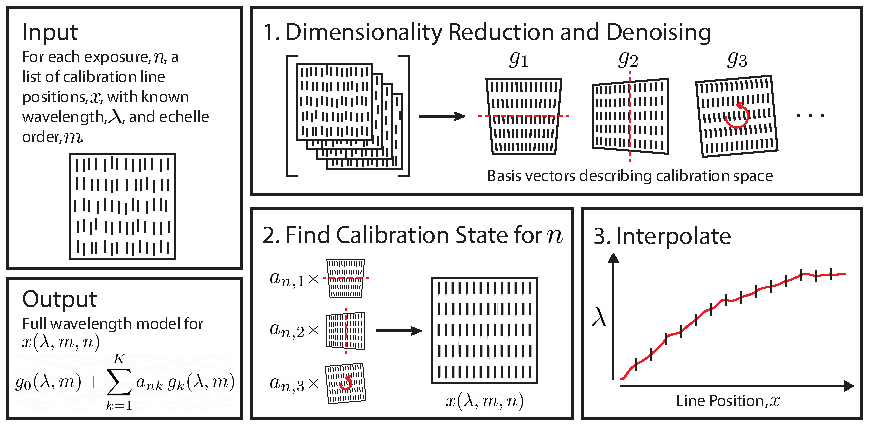
\includegraphics[width=\textwidth]{Figures/methodCartoon.pdf}
\caption{A cartoon representation of the \name\ method, as described in Section \ref{sec:method}.  We enlarge variations in measured line position, changes in calibration space, and interpolation deviations for clarity.  In step one, dimensionality reduction and denoising (\textsection \ref{sec:denoising}), the complete set of line positions for all exposures is analyzed to return a set of $K$ basis vectors, $g_n$, which represent different ways the spectrograph calibration changes.  These basis vectors span the $K$-dimensional calibration space of the spectrograph, which includes all possible wavelength solutions.  In step two (\textsection \ref{sec:interp_time}), \name\ interpolates the amplitudes of each basis vector, $a_n,k$, to return the calibration state for a specific science exposure, returned as a set of de-noised calibration lines.  The assigned wavelengths of these de-noised line positions are then interpolated onto other pixels in step three (\textsection \ref{sec:interp_wsol}) to construct a full wavelength model that returns wavelength as a function of detector position $x$ and echelle order $m$.}
\label{fig:cartoon}
\end{figure*} 

\subsection{Dimensionality Reduction: De-Noising of Calibration Frames} \label{sec:denoising}
\name\ will use calibration images to  1) determine the complete calibration space in which an instrument varies and 2) where in the accessible calibration space the spectrograph existed for each exposure.  For each calibration exposure, $n$, \name\ requires a full list of lines, $(\lambda,m)$ that are expected in each calibration exposure.  Each line is uniquely defined by a combination of echelle order, $m$, and ``true'' or theoretical wavelength, $\lambda$.  There are many strategies for identifying calibration line positions and matching them to their assigned wavelengths; this problem is left out of scope for this work.  However, we caution that systematic errors or large uncertainties in fitting line positions can propagate through to the wavelength models returned by \name.

For each exposure, $n$, every line, $(\lambda,m)$, has an associated fitted detector position, $x(\lambda,m,n)$, for example x-pixel in an 2D extracted echelle order.  Fitted line centers that are missing from an exposure (e.g. because the fit failed due to noise, the line is not in its usual echelle order, etc.) can be assigned a \code{NaN} (hardware not-a-number) for that echelle order instead.  Let there be $P$ lines per exposure.  \name\ reads in a $N \times P$ matrix of line positions for each of $P$ lines for each of $N$ exposures.

The mean of measured line position over the set of calibration exposures represents the fiducial, or standard calibration of the spectrograph, $g_0(\lambda,m)$.  In this implementation of \name, principal component analysis is performed on the difference between this fiducial calibration and each individual line position.  The returned principal components serve as basis functions,  $g_k(\lambda,m)$, expressing the possible deviations of the spectrograph from this fiducial calibration.  The magnitude of each principal component for each exposure, $a_{nk}$, represents the scalar amplitude of these deviations for each exposure.  \name\ then uses a small number, $K$, of principal components to reconstruct a de-noised version of the line positions as formulated in Equation \ref{eq:excl_wsol}.

Missing line center measurements, which were previously marked by \code{NaN}s, are replaced with de-noised estimates.  This is done iteratively until the estimates of missing line centers change by less than 0.01\%.  This process can be repeated on line centers deemed as outliers by some metric, to account for lines that may have been mis-identified or mis-fit.  The principal components from the final iteration are used to define the spectrograph's calibration space, while the associated amplitudes for each component pinpoint where in that calibration space the spectrograph is located for each calibration exposure.

\begin{algorithm}
\SetAlgoLined
\KwData{line positions $x(\lambda,m,n)$ for each exposure $n$, with wavelengths $\lambda$ and echelle orders $m$}
\KwResult{Basis vectors of the low-dimensional calibration space $g_k(\lambda,m)$, location of exposures in calibration space $a_{n,k}$}
\While{change in missing or outlier line centers $>$ 0.01\%}
{
	$g_0(\lambda,m) = \overline{x(\lambda,m,n)}$\;
	find $U, \Sigma, V$ s.t. $U\Sigma V^* = (x(\lambda,m,n)-g_0(\lambda,m))$\;
	let $a_{n,k} = U\cdot \Sigma$ and $g_k(\lambda,m) = V$\;
	$x(\lambda,m,n) = g_0(\lambda,m) + \sum_{k=1}^K a_{nk}\,g_k(\lambda,m)$ for $x(\lambda,m,n)$ = \code{NaN} where $K$ is a a small integer
	}
\caption{Dimension Reduction and De-Noising}
\end{algorithm}

\subsection{Interpolating Calibration Position}
 \label{sec:interp_time}
\name\ then interpolates the amplitude, $a_{n,k}$, of each principal component to determine the calibration state of the spectrograph.  For example, the amplitude can be interpolated with respect to time to recreate the calibration state of the spectrograph at different times.  The choice of what to interpolate against depends on the dominant contribution to variation in the calibration of the instrument.

In the implementation of \name\ presented here, the amplitudes of the principal components are interpolated linearly with respect to time.  \name\ finds new magnitudes $a_{n'k}$ for a science exposure $n'$ at time $t_{n'}$, which are used to construct the calibration state of the spectrograph for that point in time.  Using interpolated magnitudes, $a_{n,k}$, and the basis vectors, $g_k(\lambda,m)$, returned by the de-noising process, \name\ can construct a set of calibration lines, $x(\lambda,m,n') $, for any exposure as prescribed in Equation \ref{eq:excl_wsol}.


\subsection{Interpolating a Wavelength Solution} \label{sec:interp_wsol}
From the de-noising step, \name\ can now construct a set of calibration lines, $x(\lambda,m,n')$ for any exposure $n'$.  To construct a wavelength solution, \name\ interpolates the known wavelengths over the exposure specific line centers.  For instance, interpolating the known wavelengths vs. line centers onto every integer x will generate wavelengths for each pixel in an echelle order.

We found that a cubic-spline interpolation that enforces monotonicity, such as a Piecewise Cubic Hermite Interpolating Polynomial (PCHIP) interpolator, works well for interpolating wavelengths onto pixels.  A cubic spline allows for more flexibility than a continuous function, while the enforced monotonicity prevents large deviations that may befall a cubic spline.  Choice in interpolation scheme, $K$, and other tests are further discussed in Section \ref{sec:choice_wvp}.

\begin{algorithm}
\SetAlgoLined
\KwData{the fiducial calibration of the spectrograph $g_0(\lambda,m)$; magnitudes of the principal components for each exposure $a_{n,k}$; basis vectors spanning the calibration space of the spectrograph $g_k(\lambda,m)$; }
\KwResult{Wavelengths for detector positions $x'(m,n')$ of exposure $n'$ with time $t_{n'}$}

Find $a_{n',k}$ by interpolating $a_{n,k}$ with respect to $t_{n'}$\;
$x(\lambda,m,n') = g_0(\lambda,m) + \sum_{k=1}^K a_{n'k}\,g_k(\lambda,m)$ where $K=6$\;
\For{each unique $m$}{
	interpolate $\lambda$ with respect to $x(\lambda,m,n')$ onto pixels $x'(m,n')$\;
	}
\caption{Generating Wavelength Solution}
\end{algorithm}


\section{Data} \label{sec:data}
We tested \name\ using data from \expres, the EXtreme PRecison Spectrograph.  \expres\ is an environmentally-stabilized, fiber-fed, $R\sim137,000$, optical spectrograph \citep{jurgenson2016, blackman2020}.  \expres\ has two different wavelength calibration sources, a ThAr lamp and a Menlo Systems laser frequency comb (LFC).  LFCs are unique in that the wavelengths of their emission lines are stable and exactly known to the order of pico-meters  \citep{wilken2012, molaro2013, probst2014}.

Rather than using a simultaneous calibration fiber, two to three LFC exposures are interspersed between science exposures roughly every 30 minutes while the telescope is slewing to different targets.  ThAr exposures are taken at the beginning and end of each night.  All calibration data is taken through the science fiber, so that calibration light travels down the same optical pathway and is projected onto the same pixels as all science observations.

LFC lines cover echelle orders 84-124, which contain 19203 calibration lines.  Though the results are primarily based on work with LFC data, there is some discussion of applications to arc lamps.   ThAr lines cover all 86 extracted orders of \expres\ (echelle orders 75-160), which include 5295 lines.  For both the LFC and ThAr data, lines that appeared in less than 60\% of exposures were not included in the analysis.  Similarly, files with more than 60\% of expected lines missing were cut from the analysis.  

 \name\ inputs a list of echelle orders $m$, line wavelengths $\lambda$, and pixel positions $x$ of each line for each exposure.  We, therefore, use line positions generated by the pre-existing \expres\ pipeline from the following procedure \citep{petersburg2020}.
 
 A ThAr wavelength solution is generated from each ThAr exposure using the IDL code \texttt{thid.pro}, developed by Jeff Valenti.  This code identifies ThAr lines by matching lines in an exposure against a line atlas.  Lines are matched manually when there is a significant change in the instrument, but is otherwise done using forward-modeling.  Once each line's position is identified and matched to a wavelength from the line atlas, a sixth-order, 2D polynomial is fit over pixel location $x$, echelle order $m$, and scaled wavelength $m\lambda$ (wavelengths are scaled in order to distinguish lines that may appear in more than one order).
 
 Flat-relative, optimally extracted LFC data is background-corrected using a univariate spline.  Each peak in an echelle order is then fit with a Gaussian.  The mean of the fitted Gaussian is taken to be the center of the line.  For each line, the ThAr wavelength solution is used to estimate the mode number of a line.  The precise wavelength is then calculated using
 \begin{equation}
 f_n = n \times  f_r + f_0
 \label{eq:lfc}
 \end{equation}
 where the repetition rate, $f_r$, is known from design of the LFC, and the offset frequency, $f_0$, has been determined by Menlo Systems, the manufacturer of the LFC.
 
In order to satisfy the assumption of only low-order variation needed for \name, we used exposures from only one ``instrumental epoch" of \expres.  \expres\ exposures are separated into different instrumental epochs that correspond to hardware changes---changes that altered the position of the echellogram on the detector, the shape of the instrumental PSF, or the calibration sources.  Significant instrumental changes break the assumption that an  instrument will experience only low-dimensional variations, i.e. that the calibration space of all possible wavelength solutions is low-dimensional.  Each instrument epoch is therefore treated independently.  In the results presented here, we use 1227 LFC exposures and 78 ThAr exposures taken between October 14 and December 18, 2019 on 29 unique nights.


\section{Tests}\label{sec:tests}
We perform a series of tests to validate the performance of \name\ and benchmark \name -generated wavelengths against wavelengths generated by a classic, parametric method.  For all tests, we leave out a subset of calibration lines with known wavelengths as a ``validation'' sample, generate wavelengths for these lines using the remaining data, and compare the predicted wavelength to the assigned wavelength of each line.  This inherently folds in errors in the measured line center of each calibration line, but this contribution to the residuals will be the same across all tests.

To assess the classic, polynomial-driven method of wavelength calibration, we take each LFC exposure and separate the lines into even- and odd-indexed lines.  We then construct a wavelength solution using only the odd-indexed lines and use it to predict wavelengths for the even-indexed lines; i.e. a polynomial is fit to just the odd-indexed lines and then evaluated at the detector position of the even-indexed lines (see Equation \ref{eq:poly_wsol}).  We then generate a wavelength solution using only the even-indexed lines and use it to predict wavelengths for the odd-indexed lines.

To test the interpolation step of \name\ (\textsection \ref{sec:interp_wsol}), we employed \name\ on all LFC exposures with odd-indexed lines removed.  The resultant basis vectors, $g_k(x,y,m)$,  and amplitudes, $a_{nk}$, are therefore only informed by the even-indexed lines of each LFC exposure.  We then predict wavelengths for the odd-indexed lines that had been excluded and compare these predictions to their assigned wavelengths.  This allows us to test how accurately an interpolated wavelength solution can predict wavelengths.

To test the denoising step of \name\ (\textsection \ref{sec:denoising}, \textsection\ref{sec:interp_time}), we employed \name\ on a randomly selected 90\% of all LFC exposures.  This means the basis vectors, $g_k(x,y,m)$,  and weights, $a_{nk}$, were constructed using only information from 90\% of all exposures.  We used the results to predict wavelengths for all the lines in the remaining 10\% of calibration exposures.  This allows us to test how well we can pinpoint the calibration state of the spectrograph using \name.

Resultant wavelengths are compared on a line-by-line basis.  The residuals of a wavelength solution represent the difference between the wavelength solution evaluated at the line position of a calibration line, and the assigned theoretical wavelength (i.e. from Equation \ref{eq:lfc} for LFC lines and from a line atlas for ThAr lines) for each line in every exposure.  The reported RMS of a wavelength solution is therefore the per-line RMS, i.e.
\begin{equation}
RMS/line \: [m\,s^{-1}] = \sqrt{\sum_{n=1}^N\sum_{p=1}^P\frac{[ \frac{(\lambda_{n,p,predicted} - \lambda_{p,theoretical})}{\lambda_{p,theoretical}} \times c ]^2}{N \times P}}
\label{eq:rms}
\end{equation}
where $\lambda_{p,theoretical}$ is the theoretical wavelength for line $p$, $\lambda_{n,p,predicted}$ is the wavelength predicted by the constructed wavelength solution for line $p$ in exposure $n$, and residuals from all $P$ lines from all $N$ exposures are used, for a total of $N \times P$ lines.  The difference in wavelength is converted to units of $\mps$, a more intuitive metric for \eprv\ work.

\begin{figure}[t]
\centering
\includegraphics[width=.6\textwidth]{Figures/all_results.pdf}
\caption{Difference in predicted and theoretical wavelengths for the wavelength calibration tests described in Section \ref{sec:tests}.  The per line RMS as defined in Equation \ref{eq:rms} is given in the top-right corner in each method's corresponding color.  \name\ returns the smallest spread in residuals.}
\label{fig:testHists}
\end{figure} 

Histograms of the per-line residuals for each of the above described polynomial, interpolation, and denoising tests (respectively) are shown in Figure \ref{fig:testHists}.  Note that the spread in residuals is much smaller for both the denoising and interpolation tests relative to the results of the polynomial wavelength solution.

\begin{figure}[t]
\centering
\includegraphics[width=0.5\textwidth]{Figures/lineResids2D_col.png}
%\includegraphics[width=0.5\textwidth]{Figures/lineResids2D_col.pdf}
\caption{Residuals of a single LFC exposure plotted with respect to detector position (as defined by echelle order and x-pixel) for parametric and non-parametric wavelength calibration methods.  Each line is colored by the difference between the predicted wavelength and the theoretical wavelength for each line, given in units of $\mps$.  \textbf{Top}: residuals to a classic, polynomial fit.  \textbf{Bottom}: residuals to an interpolated wavelength solution.  High-order structure, i.e. vertical stripes and patchiness, is apparent in the residuals to a polynomial wavelength solution, which assumes smoothness.  The increased flexibility of the interpolated wavelength solution can account for this high-order structure, resulting in much smaller residuals with less spatial coherence.}
\label{fig:resid2d}
\end{figure}

\name -generated wavelengths also exhibit less structure in the returned residuals.  For a randomly selected example LFC exposure, Figure \ref{fig:resid2d} plots each line with respect to its echelle order (y-axis) and x-pixel on the detector (x-axis) colored by the difference between the predicted and theoretical wavelength for that line in units of $\mps$.

The residuals of the classic, polynomial wavelength solution is shown in the top plot of Figure \ref{fig:resid2d}.  There is a lot of vertical structure and some hints of a periodic, diagonal structure as well.  The residuals of the interpolation test for the same exposure is shown in the bottom plot of Figure \ref{fig:resid2d}.  There is no coherent structure here and smaller residuals.

This shows how the flexibility of an interpolated model can account for high-order instrument or detector defects, which emerged as structure in the residuals of the classic, smooth, polynomial-driven wavelength solution.  This same flexibility should similarly allow interpolated wavelength solutions to account for position errors in pixel image blocks for different detectors \citep{fischer2016, milakovic2020}.

\begin{figure}[t]
\centering
\includegraphics[width=\textwidth]{Figures/lineDensity.png}
\caption{Residuals when using ThAr lines to predict wavelengths for LFC lines.  \textbf{Right}: residuals for a single LFC exposure plotted with respect to detector position and colored by residual, as in Figure \ref{fig:resid2d}.  The positions of ThAr lines are over-plotted in yellow.  In general, residuals are greater between ThAr lines with greater separation.
\textbf{Left}: Comparison of polynomial-fit and interpolated wavelength solutions using either just ThAr lines or LFC lines for a subset of echelle order 94.  The shape of the residuals from a polynomial fit are similar whether using ThAr lines or LFC lines, suggesting that little is added with the denser LFC lines.  The LFC lines only serve to make the residuals more centered around zero.  A PCHIP interpolated wavelength model guided by LFC lines returns the smallest residuals.}
\label{fig:waveResids}
\end{figure} 

Though the interpolated wavelength solution returns lower, less-structured residuals than the polynomial wavelength solution when guided by LFC lines, the flexibility of an interpolated wavelength solution can result in much worse residuals when not properly constrained, for example in regions between widely separated calibration lines.  The left plot of Figure \ref{fig:waveResids} shows the residuals when ThAr calibration lines, which are much fewer and are less regular than LFC lines, are run through \name\ and used to predict wavelengths for the (completely independent) LFC exposures taken during the same range of time.  Over-plotted in yellow are the positions of the ThAr lines. 

Note that running \name\ informed by only ThAr lines cannot be regarded as a direct comparison to the LFC runs, as the increased uncertainty and variability in ThAr line positions alone makes the resultant wavelength predictions an order of magnitude worse, hence the different scale of the colorbar in the left plot of Figure \ref{fig:waveResids} as compared to Figure \ref{fig:resid2d}.  All the same, the residuals are in general worse where lines are further apart (for example, in redder echelle orders) than where lines are denser.

Figure \ref{fig:waveResids} plots the residuals for a subset of order 94 for both a polynomial-based method and a PCHIP-based method guided by either ThAr lines or LFC lines.   The PCHIP model with ThAr lines (orange curve) returns huge residuals between two widely-separated ThAr lines that extends out of frame.  The classic, polynomial fit exhibits similar residuals in both amplitude and shape regardless of whether the set of ThAr lines or LFC lines are used.  An interpolated wavelength solution using LFC lines (black curve) exhibits the lowest residuals.

The move to an interpolated wavelength solution is driven by the assumption that a high density of calibration lines allows for more freedom in the resultant wavelength solution.  This freedom allows the wavelength solution to more accurately ascribe wavelengths.  This flexibility, however, is no longer justified in the regime where there are large separations between calibration lines, as this no longer provide sufficient constraint on the interpolated wavelength solution, as is the case in some regions of a classic ThAr lamp.

\subsection{Impact on Radial Velocity Measurements}\label{sec:test-rv}
We tested the effect of \name -generated wavelengths on RV measurements using \expres\ observations of \target.  \target\ is a BLANK star and also SOME STATEMENT ON SUSPECTED ACTIVITY(?).  We used BLANK observations of \target\ taken between BLANK and BLANK with an average signal-to-noise ratio of BLANK PROBABLY 250.  Radial velocity mesurements are derived using a chunk-by-chunk, forward-modeling algorithm employed by \expres's pipeline \citep{petersburg2020}.

Figure \ref{fig:rvs} compares the resultant RVs when using a classic, ninth-degree polynomial wavelength solution and an \name -generated wavelength model.
\lz{Awaiting latest extraction run...}


\section{Choose Your Own Implementation} \label{sec:choices}
We have described and tested only one implementation of \name.  Using PCA and an interpolated wavelength solution is a statisticall straight-forward step towards a complete hierarchical and non-parametric wavelength model.  It is possible to upgrade both the denoising and wavelength solution steps to true models.  It is also possible, of course, to implement either step individually.  A hierarchical framework can be used to simply denoise the lines before they are fit to a parametric model, or use a non-parametric model on lines that haven't been denoised.

\lz{Hogg: please edit/add to these methods}

For the dimensionality reduction and denoising, the PCA could be replaced by a probabilistic PCA model or other probabilistic linear reduction methods.  It is also possible to move to non-linear reduction methods, like...?

The wavelength solution could also move past interpolation.  For example, a Gaussian process could be used that is constrained to ensure monotonicity.  Replacing each step with a model will allow for full, hierarchical Bayesian inference.  This means the uncertainty from wavelength calibration could be completely marginalized out.  Doing so will have the largest impact if the wavelength calibration is a significant fraction of the error budget.

The implementation of \name\ presented here, using PCA for denoising and interpolating a wavelength solution, uses various global variables and methods that we believe are or are close to optimal for constructing a high-fidelity wavelength solution.  The following subsections will describe each choice and the associated decision-making process.

\subsection{Value of K}
\label{sec:choice_k}
The value of $K$ represents the dimensionality of the calibration space within which the spectrograph lives.  In practice, it is the number of principal components, or basis vectors, used to reconstruct the de-noised line centers.  $K$ needs to be large enough so that all variability in the spectrograph is captured.  Too large, however, and the reconstruction will begin to incorporate noise, thereby defeating the purpose.

\begin{figure}[h]
\centering
\includegraphics[width=.5\textwidth]{Figures/kvals_all.pdf}
\caption{Per-line RMS of returned wavelength models for different values of $K$.  Per-line RMS is defined in Equation \ref{eq:rms} and provides a measure of the accuracy of a wavelength model.  There is a dotted, vertical line at $K=6$, our chosen $K$ value.  The dotted, horizontal line is the RMS for $K=6$.  The improvement at around $K=6$ plateaus.}
\label{fig:kvals}
\end{figure}

\begin{figure*}[t]
\centering
\includegraphics[width=\textwidth]{Figures/pcsLfc9.png}
%\includegraphics[width=\textwidth]{Figures/pcsLfc6.pdf}
\caption{\textbf{Top}:  The fiducial calibration of the spectrograph, i.e. the mean line positions for each line throughout the epoch of stability.  The following $3 \times 3$ grid of plots show the first nine principal components constructed using LFC lines.  These principal components represent the basis vectors along which the calibration of the spectrograph can deviate from the fiducial calibration.  For each principal component, or basis vector, each calibration line is plotted according to its echelle order and x-pixel and colored by the value of the basis vector for that line.  Principal components beyond the sixth one become steadily more dominated by noise.}
\label{fig:pcLfc}
\end{figure*}

In deciding a $K$ value, we ran denoising tests, as described in Section \ref{sec:tests}, for $K$ values spanning from 2 to 512.  The resultant per-line RMS for each test is plotted in Figure \ref{fig:kvals}.  One would expect the returned wavelengths to get increasingly more accurate with larger $K$ until components that represent only noise are incorporated.  Residuals might then get worse before ultimately starting to get better again with large $K$, which marks the model over-fitting the data.  Though the returned RMS never gets worse, we find that the improvement plateaus between $K=6$ and $K=128$.  Comparisons of wavelengths returned by a $K=6$ model vs. a $K=32$ model show significant differences in less than 10 bluer lines, which are known to have greater error and variance in their measured line positions.  We therefore settled on a $K$ value of six.

Figure \ref{fig:pcLfc} shows the fiducial calibration state and the first 9 principal components constructed using LFC lines, which represent deviations from the fiducial calibration state.  There is clear structure in the first and second principal components.  Components three through six show smaller or more localized structure.  Components three and four have aberrant behavior on the edges of the two bluest echelle orders, where lower signal results in more variation in the line fits.  Later principal components become dominated by noise and show less coherent structure.
\pagebreak
\subsection{Interpolation of Calibration State to Science Exposures}
\label{sec:choice_avt}
Figure \ref{fig:nightlyVariation} shows the amplitude of the first and second principal component with respect to time on the left.  Though there exists a complex overall shape to the amplitudes with respect to time, a clear linear trend exists within each night.  This is shown by the right plots in Figure  \ref{fig:nightlyVariation}.  As the beginning-of-night and end-of-night calibration sets always include LFC exposures, we use a simple linear interpolation to interpolate principal component amplitudes with respect to time.

\begin{figure*}[t]
\centering
\includegraphics[width=\textwidth]{Figures/pcAs_byDay.png}
\caption{Amplitude of the first two principal components shown as a function of time (left) or hour from midnight (right).  The top row of plots shows the amplitudes for the first principal component while the bottom row shows the amplitudes for the second principal component.  Lines show the result of a linear interpolation.  In the top, right plot, the temperature of the optical bench is also plotted in orange.  In the right plot, the principal component amplitudes have been artificially offset by the median amplitude for each night.  All days are therefore roughly on the same scale, but the y-axis is different from the left plots.  In the right column, points are colored by the MJD of each exposure.}
\label{fig:nightlyVariation}
\end{figure*} 

The choice in interpolation method can help guide how many wavelength calibration images are truly needed.  It is unnecessary to take calibration images at times where the same information can be constructed by a well-chosen interpolation scheme.  For example, with the \expres\ data shown here, it is clear that nightly calibration images are needed, but for a linear trend, only two calibration images throughout the night are strictly required.

The amplitudes $a_{n,k}$ can also be interpolated with respect to any good housekeeping data, not just time.  Best results will come from interpolating with respect to whatever is most strongly correlated with the calibration state of the spectrograph.  For example, with \expres, which is passively temperature controlled, the returned amplitudes $a_{n,k}$ were extremely correlated with the optical bench temperature, as shown in Figure \ref{fig:nightlyVariation}, suggesting it would also be possible to interpolate the amplitudes with respect to temperature.

Another pertinent example would be a spectrograph that is mounted on the telescope, and therefore moves with the telescope.  In this case, it may be important to interpolate at least in part with respect to the position of the telescope, which enables the resultant calibration to incorporate the gravitational loading experienced by the spectrograph.


\subsection{Interpolation of Wavelengths with Respect to Pixel}
\label{sec:choice_wvp}
In the implementation described here, interpolation of wavelengths over pixel  is done order by order using a Piecewise Cubic Hermite Interpolating Polynomial (PCHIP) interpolator.  This interpolation incorporates the flexibility needed to model the changing dispersion of the spectrograph across an echelle order along with any detector defects while also enforcing monotonicity, which we know must be true across any one echelle order.

A simple linear interpolation would give erroneously low values everywhere.  Due to the dispersion intrinsic to echelle spectrographs, the wavelength change between pixels grows greater with greater wavelengths.  This means that the function of wavelength vs. pixel across an echelle order will always be monotonically increasing and concave down everywhere.

A more classic cubic spline interpolation can run into issues with arc lines, which are irregularly spaced or even blended.  Close lines appearing at virtually the same pixel location but with different wavelengths could coerce a cubic spline into a very high slope, as with the green curve in Figure \ref{fig:xinterp}.  A line blend appears at approximately pixel 5300, causing the spline to twist to nearly vertical to account for both points.  This leads to huge deviations from the correct wavelengths around this line blend as the extraneously high slope of the spline is accounted for.

\begin{figure*}[t]
\centering
\includegraphics[width=\textwidth]{Figures/intpx_tests.png}
\caption{Residuals from different interpolation schemes over pixels in echelle order 100.  ThAr lines, shown as blue circles, are used to construct a wavelength solution that is then evaluated at each LFC line, shown as blue lines.  The residuals of each wavelength solution for a subset of the order is shown on the left.  Histograms of the residuals for each method for the complete order is shown on the right.  Here, the y-axis is zoomed in to show the shape of each histogram more clearly.  Note: there is a blended ThAr line at approximately pixel 5300, the last ThAr line plotted.}
\label{fig:xinterp}
\end{figure*} 

These huge digressions can be avoided by allowing for some smoothing in the interpolation.  In Figure \ref{fig:xinterp}, we show an example in orange using SciPy's implementation of a univarate spline.  While the result appears to follow the calibration lines much better, the smoothing ultimately causes larger residuals that are spatially correlated (Fig. \ref{fig:xinterp}, right).  In all echelle orders, the edges are overestimated while the middle will be underestimated, shown by the flattened shape of the histogram of residuals.  The resultant wavelength solution is underestimating the curvature of the pixel-wavelength relation, giving rise to similar issues as with an inflexible, parametric wavelength solution.  Introducing this smoothing parameter is enforcing a smoothness we have no reason to believe is true of the data, thereby re-introducing one of the problems with parametric models.

We instead turn to the PCHIP interpolator, which damps down huge deviations in the traditional cubic spline by requiring the resulting interpolated function be monotonic.  Monotonicity is a constraint we know must be true for any one echelle order.  Though the PCHIP interpolator shows a similar issue as a classic cubic spline around the ThAr line blend at pixel 5300, the effect is much smaller and effects fewer pixels.  Figure \ref{fig:xinterp} shows that using the PCHIP interpolator returns the lowest residuals.  


\section{Application to Other Spectrographs}
\label{sec:others}
We focus on an \eprv\ use-case here, because there is a strong need for wavelength calibration in the \eprv\ community.  \expres\ is representative of the newest generation of \eprv\ spectrographs, and an LFC provides stable, dense calibration lines with known wavelengths, ideal for \name.  The applicability of \name\ to any one instrument is a detailed question of the kind of variance experienced by the spectrograph and calibration sources available, but we hope to provide some approximate benchmarks and diagnostics.

Implementing \name\ will require an existing library of calibration exposures that span the range of calibration space accessible by the spectrograph, or at least the space accessed by the science exposures being calibrated.  A new set of calibration exposures would be needed for any changes to the instrument that could significantly change the calibration space.  While there is no exact cutoff for how many exposures are needed, the number is certainly much larger than $K$, the dimensionality of the calibration space.  More calibration exposures will help with denoising .  The number of calibration exposures required throughout a night will depend on how much the instrument varies throughout the night, and the chosen interpolation scheme, as mentioned in Section \ref{sec:choice_avt}.

As an empirical assessment of the needed line density, we systematically removed LFC lines from the \expres\ data and calculated the per-line RMS of the returned wavelengths for the removed lines.  Figure \ref{fig:density} plots the scatter of residuals of the wavelengths returned by \name\ as a function of separation between lines in units of resolution element.  It gives an approximate estimation of the expected error between lines of different separation.  Note, however, that the stability of the lines and their measured line centers quickly becomes the dominant error source in calibration lamps over the separation between lines.  The needed line density depends on the resolution of a given spectrograph and the needed precision of the returned wavelength solution.

\begin{figure}[h]
\centering
\includegraphics[width=0.5\textwidth]{Figures/lfcDensityTest.pdf}
\caption{Per-line RMS as a function of spacing between lines in units of resolution element.  The average line spacing is calculated using the average distance between LFC lines across its wavelength range.}
\label{fig:density}
\end{figure} 

\name\ can easily incorporate simultaneous calibration data, where a calibration source is taken through a reference fiber during science exposures, especially if the simultaneous reference is also used when taking calibration images.  The position of calibration lines taken through the reference fiber can simply be concatenated to the array of line positions taken through the science fiber.  Both sets of lines when then be used when the low-dimensional basis is constructed.  This allows the simultaneous calibration information to contribute to constructing the complete calibration space of the spectrograph and pinpoint where the spectrograph is in that calibration space for any exposure.

The calibration for any science exposure with a simultaneous reference can be determined by finding the amplitude of each basis vector that most closely recreates the calibration line positions through the reference fiber.  These amplitudes can then be used to recreate the calibration line positions through the science fiber as well.  This replaces the need to interpolate the basis vector amplitudes from calibration exposures to science exposures, something that is done with respect to time in the example implementation described in this paper.  The result is likely to be even more precise, as this method incorporates more data.

It is also possible to apply \name\ to etalon data with some modifications.  The simplest implementation is if the free spectral range (FSR) and therefore wavelength of each line of the etalon is well known.  The etalon data can be interpolated onto a set of fiducial lines with set wavelengths.  These fiducial lines would therefore be identifiable by echelle order and wavelength alone, with only their line positions varying with different exposures, thereby returning to the same framework as developed for the case of an LFC.  This marks the simplest implementation of \name\ on etalon data, as the uncertainty of a line's wavelength is upstream of the model rather than built in.

\lz{Hogg: The following paragraph might need some work.  I struggled to keep this discussion general (i.e. not referring to our specific implementation of \name) while also being helpful.  However, I might have failed or just made all this very confusing.  What do you think?}

If the FSR varies very little, its value can in principle be captured by a PCA or similar method.  However, to interpolate this information from calibration exposures to science exposures would necessitate a simultaneous reference or interpolation with respect to some other housekeeping data that contains information on the value of the FSR.  If the FSR varies a lot, it becomes untenable to capture these changes with a PCA or similar method.  Instead, the resultant basis vectors of the calibration space would have to be conditioned on the value of the FSR, becoming a non-trivial extension of \name.

In terms of dimensionality reduction, most physical systems should have only a few dominant axis along which they vary, meaning \name\ should be adaptable to a wide range of instrument designs.  With PCA, this can be tested by plotting the amplitude of the returned principal components, which should fall quickly after a few components.  However, this only provides a measure of the variance in the PCA space, and is not an explicit test of the end-to-end variation in the resulting model.  This condition is therefore necessary but not sufficient if implementing \name\ with PCA.

It could still be possible to run \name\ on a spectrograph that has a high-dimensional calibration space, meaning a large number of basis vectors is required to capture all the variance in the spectrograph.  In this regime, there is always the risk of over-fitting.  Regularizing the principal component amplitudes, for example insisting the amplitudes for higher principal components be smaller, can help to return reasonable models \citep{formanmackey2015} .  Within such a framework, \name\ may still deliver good results.
\lz{Hogg: My notes said you might want to add more things here?}

For the results presented here, the data was broken up into different eras of stability based on where the principal component amplitudes showed huge deviations.  This was done visually, though there exists many change-point detection algorithms that could be used \citep{aminikhanghahi2017}.  There is a trade-off in including more exposures between introducing greater variation, but also more data to offer constraints that may be optimized.  Here, an era of stability was chosen  manually in order to focus on separating out time-domain intervals in which the data is relatively homogeneous, e.g. most exposures show the same calibration lines.  Homogeneity is, of course, implicitly required when implementing PCA.

Lastly, we caution that \name\ is extremely sensitive to upstream changes, for example an unstable PSF or slanting slit function, that may effect the line centers.  For example, PCA is good for detecting variability, but is agnostic to the source of the variability.  This is why the principal components shown in Figure \ref{fig:pcLfc} exhibit errant values for bluer LFC lines, which are lower signal and therefore have more variable fitted line centers.  It is essential that the line positions being given to \name\ capture only the changes in the spectrograph's calibration state, not potential errors in the fitted line centers. 


\section{Discussion} \label{sec:discussion}
We show that \name\ returns a lower per-line RMS than classic, parametric methods by a factor of 5 (Section \ref{sec:tests}).  The residuals were also smoother, showing less spatial correlation.  Using \name\ wavelengths also reduced the RMS in a planet fit to derived RVs by \lz{some percent hopefully probs} (Section \ref{sec:test-rv}).  In implementing \name\ on \expres\ data, we have successfully constructed a model of \expres, which truly is an instrument with low-degrees of freedom.  \name\ does not make any claims about what variability each basis vector represents.  Those interested in interpreting the variability are encouraged to investigate how the amplitude of the different vectors varies with different housekeeping data to find their source.

The endeavor to reach $0.1\,\mps$ radial-velocity precision necessitates improvements on all levels of spectroscopy, from the instrumentation to the data analysis.  We believe implementing \name, a hierarchical, non-parametric model for wavelength calibration, is a step towards reducing the error contribution from data reduction pipelines.

Starting with a list of calibration lines with known wavelengths and well-fit line centers for each calibration exposure, \name\ will de-noise and interpolate the given lines into a full wavelength solution.  \name\ levies the stability of contemporary EPRV instruments and high density of lines made available by new calibration sources, such as LFCs and etalons, to achieve more accurate wavelengths.  \name\ therefore assumes dense enough calibration lines to properly constrain a non-parametric wavelength model, and that the instrument has low degrees of freedom.

Denser calibration lines allow us to move to more flexible wavelength models that can account for non-smooth features in the wavelength solution.  Stabilized spectrograph hardware makes it more likely that the calibration state of the instrument is low-dimensional.  All calibration images in a given generation of stability can therefore be used to constrain the accessible calibration space of the spectrograph as well as where in that calibration space the spectrograph lies for each calibration exposures.  We have described only one, fairly simplistic implementation of \name\ here.  There are many options for both the de-noising and interpolation steps, as mentioned in Section \ref{sec:choices}.

An advantage of this implementation, where PCA is applied to line positions from all LFC exposures, is the ability to isolate exposures that exhibit errant variation, which is typically associated with flawed exposures.  This allowed us to quickly vet for problematic LFC exposures, which otherwise would have required visual inspection of all 1200+ LFC exposures.  In a classic framework where each calibration exposure is treated independently, these aberrant exposures would likely have persisted undetected and would likely have swayed the resultant wavelength solutions for at least an entire night.

On the other hand, PCA captures all variance, regardless of source.  Though \name\ endeavors to capture only variation in the instrument, the PCA is also sensitive to uncertainties and failures in the upstream line position fitting.  For example, we have seen that lower-signal lines that are harder to fit faithfully will have greater variety in returned line positions, which is in turn captured by the PCA.  In this sense, \name\ is actually a model of not just the instrument, but all the upstream choices used to drive live positions.  High-fidelity line positions are essential to ensure the PCA is capturing variations in just the spectrograph's calibration rather than changes in how well a line can be fit or other effects.

\lz{Hogg: I'm still not sure I completely grasp the issue, can this be made clearer?}
Along those lines, we caution that with any wavelength solution, there is a perfect degeneracy between what is defined as the ``position of the line'' and the resultant wavelength solution.  If, for example, a cross correlation method is used to extract RVs from the data, a systematic difference may be introduced depending on the definition of what exactly is the line position, whether it be the center of a Gaussian fit, the edge of a complicated PSF, etc.  In principle, the best way to mitigate this uncertainty would be to use a calibration source that looks like a star.

Compared to traditional methods, which involve fitting high-order polynomials, \name\ has several useful statistical properties.  \name\ is technically robust to localized issues with either the calibration source or the pipeline used to return line positions.  With an interpolated wavelength model, one errant line position will only effect the resultant wavelength model out to the close, neighboring lines.  The effect of an outlier is diminished and kept localized.  In contrast, an entire parametric fit will change from a single errant line, changing the wavelength solution for the entire exposure for a 2D fit.  Through de-noising and outlier rejection, \name\ adds additional robustness against erroneous line positions.

The locality of the interpolation caries other benefits as well.  Manufacturing artifacts in the detector or other optical elements can lead to non-smooth structure in the wavelength solution that can not be captured by polynomials or other smooth functions (see \figurename~\ref{fig:resid2d}).  An interpolated model introduces greater flexibility, enabling the model to account for such high-order effects.  As discussed in Section \ref{sec:choice_wvp}, there are better and worse interpolators for the task, which may differ for different instruments and different calibration sources.  Instead of using an interpolator at all, there might be better results from implementing something more sophisticated, such as a kernel method or a Gaussian process with a kernel adapted for the specifics of an instrument.  There is in principle an enormous number of non-parametric methods to explore, which we leave outside the scope of this paper.

Similarly, PCA is just one of many possible dimensionality-reduction methods.  We chose to implement \name\ using PCA here for simplicity and computational tractability.  If \name\ was updated to a full probabilistic model, the PCA along with the interpolation model would have to be upgraded to something with better probabilistic properties.  Further discussion of other implementations of \name\ can be found in Section \ref{sec:choices}.

\name\ can be applied to any data that contains information about the calibration state of the spectrograph (see Section \ref{sec:others}).  For example, though LFC and ThAr exposures are used as an example in this paper, \name\ would work similarly for an etalon or any other arc lamp with a list of lines and assigned wavelengths.  Simultaneous calibration information can easily be accounted for by simply including the line position information from the simultaneous reference when constructing a low-dimensional basis of the instrument's calibration space.

Once we have defined a calibration space that captures all possible degrees of freedom for a stabilized spectrograph, there are many options for pinpointing where the spectrograph is located within that calibration space.  Good housekeeping data, such as temperature or pressure could be used in addition to or instead of time (as mentioned in Section \ref{sec:choice_avt}).  Telemetry that is seen to be correlated with the calibration state of the spectrograph can even be added to the data used to construct the low-dimensional basis.  Furthermore, all exposures taken with the spectrograph in principle contains information about the calibration state of the spectrograph.  Theoretically, tellurics, lines in science exposures, or just the trace positions themselves could also be used to determine an instrument's calibration state, negating the need for any additional wavelength-calibration source beyond defining the calibration space.

\name\ is designed and optimized for extreme-precision, radial-velocity spectrographs.  In the battle to construct a high-fidelity data pipeline for extreme-precision radial-velocity measurements, we believe \name\ represents a step towards mitigating the error from wavelength calibration, as demonstrated by tests using \expres\ data (Section \ref{sec:tests}).  Though the focus was on \eprv\ instruments here, \name\ should be largely applicable to nearly any astronomical spectrograph.

\software{SciPy library \citep{scipy}, NumPy \citep{numpy, numpy2}, Astropy \citep{astropy:2013,astropy:2018}.}

\facilities{LDT}

\acknowledgements{We thank the EXPRES team for their work on the instrument, software, and pipeline.  We thank Dan Foreman-Mackey for illuminating discussion.  The data presented here made use of the Lowell Discovery Telescope at Lowell Observatory. Lowell is a private, non-profit institution dedicated to astrophysical research and public appreciation of astronomy and operates the LDT in partnership with Boston University, the University of Maryland, the University of Toledo, Northern Arizona University and Yale University. We gratefully acknowledge ongoing support for telescope time from Yale University, the Heising-Simons Foundation, and an anonymous donor in the Yale community. We especially thank the NSF for funding that allowed for precise wavelength calibration and software pipelines through NSF ATI-1509436 and NSF AST-1616086 and for the construction of EXPRES through MRI-1429365.  LLZ gratefully acknowledges support from the National Science Foundation Graduate Research Fellowship under Grant No. DGE1122492.}

\bibliography{paper.bib}

\end{document}
